\documentclass[a4paper,14pt]{extarticle}

\usepackage[utf8x]{inputenc}
\usepackage[T1]{fontenc}
\usepackage[russian]{babel}
\usepackage{hyperref}
\usepackage{indentfirst}
\usepackage{here}
\usepackage{array}
\usepackage{graphicx}
\usepackage{caption}
\usepackage{subcaption}
\usepackage{chngcntr}
\usepackage{amsmath}
\usepackage{amssymb}
\usepackage[left=2cm,right=2cm,top=2cm,bottom=2cm,bindingoffset=0cm]{geometry}
\usepackage{multicol}
\usepackage{multirow}
\usepackage{titlesec}
\usepackage{listings}
\usepackage{color}
\usepackage{enumitem}
\usepackage{cmap}
\usepackage{underscore}

\definecolor{green}{rgb}{0,0.6,0}
\definecolor{gray}{rgb}{0.5,0.5,0.5}
\definecolor{purple}{rgb}{0.58,0,0.82}

\lstdefinelanguage{none}{}

\lstset{
	language={C++},
	inputpath={../generator/src/main/java/com/vaddya/hotelbooking},
	backgroundcolor=\color{white},
	commentstyle=\color{green},
	keywordstyle=\color{blue},
	numberstyle=\scriptsize\color{gray},
	stringstyle=\color{purple},
	basicstyle=\ttfamily\small,
	breakatwhitespace=false,
	breaklines=true,
	captionpos=b,
	keepspaces=true,
	numbers=left,
	numbersep=5pt,
	showspaces=false,
	showstringspaces=false,
	showtabs=false,
	tabsize=4,
	texcl=true,
	extendedchars=false,
	frame=single,
	morekeywords={IF, BIGSERIAL, SERIAL, TEXT, BIGINT, MONEY, BOOLEAN, REFERENCES}
}

\renewcommand{\le}{\ensuremath{\leqslant}}
\renewcommand{\leq}{\ensuremath{\leqslant}}
\renewcommand{\ge}{\ensuremath{\geqslant}}
\renewcommand{\geq}{\ensuremath{\geqslant}}
\renewcommand{\epsilon}{\ensuremath{\varepsilon}}
\renewcommand{\phi}{\ensuremath{\varphi}}
\renewcommand{\thefigure}{\arabic{figure}}
\newcommand{\code}[1]{\texttt{#1}}
\newcommand{\caret}{\^{}}

\titleformat*{\section}{\large\bfseries} 
\titleformat*{\subsection}{\normalsize\bfseries} 
\titleformat*{\subsubsection}{\normalsize\bfseries} 
\titleformat*{\paragraph}{\normalsize\bfseries} 
\titleformat*{\subparagraph}{\normalsize\bfseries} 

\counterwithin{figure}{section}
\counterwithin{equation}{section}
\counterwithin{table}{section}
\newcommand{\sign}[1][5cm]{\makebox[#1]{\hrulefill}}
\newcommand{\equipollence}{\quad\Leftrightarrow\quad}
\newcommand{\no}[1]{\overline{#1}}
\graphicspath{{../pics/}}
\captionsetup{justification=centering,margin=1cm}
\def\arraystretch{1.3}
\setlength\parindent{5ex}
\titlelabel{\thetitle.\quad}

\setitemize{topsep=0.3em, itemsep=0em}
\setenumerate{topsep=0.3em, itemsep=0em}

\begin{document}

\begin{titlepage}
\begin{center}
	Санкт-Петербургский Политехнический Университет Петра Великого\\[0.3cm]
	Институт компьютерных наук и технологий \\[0.3cm]
	Кафедра компьютерных систем и программных технологий\\[4cm]
	
	\textbf{ОТЧЕТ}\\ 
	\textbf{по лабораторной работе}\\[0.5cm]
	\textbf{<<Изучение прикладных протоколов в командной строке Linux>>}\\[0.1cm]
	Разработка сетевых приложений\\[3.0cm]
\end{center}

\begin{flushright}
	\begin{minipage}{0.45\textwidth}
		\textbf{Работу выполнил студент}\\[3mm]
		группа 43501/3 \hfill Дьячков В.В.\\[5mm]
		\textbf{Работу принял преподаватель}\\[5mm]
		\sign[3cm] \hfill Зозуля А.В. \\[5mm]
	\end{minipage}
\end{flushright}

\vfill

\begin{center}
	Санкт-Петербург\\[0.3cm]
	\the\year
\end{center}
\end{titlepage}

\addtocounter{page}{1}

\tableofcontents
\newpage

\section{Цель работы}

Исследовать возможности анализаторов трафика на примере бесплатного и свободно распространяемого инструмента WireShark.

\section{Программа работы}

\begin{enumerate}
	\item Анализ пакетов ARP-запроса и ARP-ответа.
	\item Анализ ICMP пакетов:
		\begin{itemize}
			\item с использованием утилиты \code{ping};
			\item с использование фрагментации пакетов в утилите \code{ping};
			\item с использованием утилиты \code{traceroute};
			\item получение и анализ ошибок.
		\end{itemize}
	\item Анализ UDP пакетов.
	\item Анализ TCP пакетов:
		\begin{itemize}
			\item установление соединения;
			\item разрыв соединения;
			\item сброс соединения.
		\end{itemize}
\end{enumerate}

\section{Сведения о компьютере}

Для вывода информации о системе используем утилиту \code{uname}:
\lstinputlisting{uname.txt}

Для получения информация о состоянии активных интерфейсов была использована UNIX-утилита \code{ifconfig}:
\lstinputlisting{ifconfig.txt}

\vspace{-1em}
\section{Протокол ARP}

\subsection{Теоретическая информация}

Протокол ARP (Address Resolution Protocol, протокол разрешения адресов), описанный в RFC 826 , используется для определения соответствия между логическим адресом сетевого уровня (IP) и физическим адресом устройства (MAC). 

ARP состоит из двух частей. Первая – определяет физический адрес при посылке пакета, вторая – отвечает на запросы других станций.

Протокол имеет буферную память (ARP-таблицу), в которой хранятся пары адресов (IP-адрес, MAC-адрес) с целью уменьшения количества посылаемых запросов, следовательно, экономии трафика и ресурсов.

Выведем содержимое ARP-таблицы:
\lstinputlisting{arp/list.txt}

Видно, что в arp-таблице только одна запись, соответствующая маршрутизатору.  Формат ARP-сообщения:

\begin{itemize}
	\item тип сети (16 бит): для Ethernet -- 1;
	\item тип протокола (16 бит): 0800h для IP;
	\item длина аппаратного адреса (8 бит);
	\item длина сетевого адреса (8 бит);
	\item тип операции (16 бит): 1 -- запрос, 2 -- ответ;
	\item аппаратный адрес отправителя (переменная длина);
	\item сетевой адрес отправителя (переменная длина);
	\item аппаратный адрес получателя (переменная длина);
	\item сетевой адрес получателя (переменная длина).
\end{itemize}

\subsection{Захват и анализ трафика}

Удалим существующую запись из ARP-таблицы, установим фильтр захвата -- \code{arp} и захватим отправляемые и получаемые пакеты после этого. 

Широковещательный ARP-запрос для определения MAC-адреса устройства с IP-адресом \code{192.168.1.1}:
\screen{arp/arp_request}

ARP-ответ от Tp-Link (маршрутизатор) с IP-адресом \code{192.168.1.1}, содержащий искомый MAC-адрес:
\screen{arp/arp_response}

Видно, что ARP-ответ не является широковещательным.

\section{Протокол ICMP}

\subsection{Теоретическая информация}

ICMP (Internet Control Message Protocol, протокол межсетевых управляющих сообщений) -- сетевой протокол, входящий в стек протоколов TCP/IP. В основном ICMP используется для передачи сообщений об ошибках и других исключительных ситуациях, возникших при передаче данных, например, запрашиваемая услуга недоступна, или хост, или маршрутизатор не отвечают. Также на ICMP возлагаются некоторые сервисные функции.

\subsection{Утилита \code{ping}}

Утилита \code{ping} служит для проверки возможности доставки IP-пакетов и использует ICMP-сообщения с типом 8 (эхо-запрос) и 0 (эхо-ответ).

Выполним \code{ping ya.ru} и захватим пакеты. Был отправлен ping-запрос:
\screen{icmp/ping_request}

\newpage

Был получен ping-ответ:
\screen{icmp/ping_response}

Таким образом был отправлен ping-запрос (ICMP пакет с типом 8) и получен ping-ответ (ICMP пакет с типом 0).

Укажем размера пакетов утилите \code{ping} с использованием ключа \code{-s 4000} и выполним захват всех IP-пакетов.

Был отправлен фрагментированный ping-запрос. Видно, что 4 КБ запрос был разбит на 3 пакета размером 1514 Б, 1514 Б и 1002 Б соответственно, то есть 4030 Б в сумме (объясняется добавлением заголовков). Кроме того, ICMP-заголовок присутствует только в первом пакете и поэтому WireShark не определяет остальные пакеты как ICMP-запросы. Кроме того, в фрагментированных пакетах добавляются флаги в IP-заголовок, содержащие информацию о фрагментации.
\screen{icmp/ping_fragmented_request_1}
\screen{icmp/ping_fragmented_request_2}

Был получен фрагментированный ping-ответ. Видно, что было получено 5 пакетов, то есть ответ был также фрагментирован. Ping-ответ должен содержать данные, полностью совпадающие с данными, отправленными в запросе. Аналогично запросу, пакеты содержат флаги с информацией о фрагментации.
\screen{icmp/ping_fragmented_response_1}
\screen{icmp/ping_fragmented_response_2}

\subsection{Утилита \code{traceroute}}

Утилита \code{traceroute} отображает путь следования IP-пакетов и использует ICMP-сообщения с типом 11. Запустим \code{traceroute} для определения маршрута до сервера \code{ya.ru}. Для использования ICMP пакетов необходим ключ \code{-I} (необходимы права суперпользователя):

\lstinputlisting{icmp/traceroute.txt}

\screen{icmp/traceroute_1}
\vspace{-2.2em}
\screen{icmp/traceroute_2}

Для определения промежуточных маршрутизаторов \code{traceroute} отправляет целевому узлу серию ICMP-пакетов (по умолчанию 3 пакета), с каждым шагом увеличивая значение поля TTL («время жизни») на 1. Первая серия пакетов отправляется с TTL, равным 1, и поэтому первый же маршрутизатор возвращает обратно ICMP-сообщение <<time exceeded in transit>>, указывающее на невозможность доставки данных. Утилита фиксирует адрес маршрутизатора, а также время между отправкой пакета и получением ответа (эти сведения выводятся на монитор компьютера). Затем \code{traceroute} повторяет отправку серии пакетов, но уже с TTL, равным 2. Процесс повторяется до тех пор, пока пакет не достигнет целевого узла. При получении ответа от этого узла процесс трассировки считается завершённым.

\subsection{Получение ICMP ошибок}

Отправим ping-запрос на IP-адрес \code{10.1.17.3}, чтобы получить сообщение об ошибке.

\lstinputlisting{icmp/error.txt}

\screen{icmp/error}

Видно, что был получен ICMP-ответ, содержащий тип 3 (Destination Unreachable) и код 1 (Destination host unreachable). Такой ответ генерирует маршрутизатор, который находится в одной сети с адресом назначения, но при этом хост с таким адресом недоступен (не отвечает на ARP-запросы).

\newpage

\section{Протокол UDP}

UDP (User Datagram Protocol) -- один из ключевых элементов TCP/IP, работающий поверх сетевого протокола IP. Он является простым и ориентирован на передачу дейтаграмм. Захватим DNS-запрос как пример UDP-пакета. Для этого снова выполним \code{ping ya.ru}.

\screen{udp/dns}

Видно, что в IP-заголовке указан протокол UDP, а UDP-заголовок содержит порт отправителя (выданный ОС порт 46382) и получателя (используемый DNS порт 53), длину датаграммы (42 байта) и контрольную сумму.

\section{Протокол TCP}

Transmission Control Protocol (TCP, протокол управления передачей) -- один из основных протоколов передачи данных интернета, предназначенный для управления передачей данных. В стеке протоколов TCP/IP выполняет функции транспортного уровня модели OSI.

В заголовке IP-пакета указывается протокол TCP. В качестве TCP-сервера для экспериментов используем \code{example.com} и с помощью \code{telnet} будем подключаться к 80-ому порту.

\subsection{Установление соединения}

Процесс начала сеанса TCP (также называемый <<рукопожатие>>, handshake), состоит из трёх шагов:

\begin{enumerate}
	\item Клиент, который намеревается установить соединение, посылает серверу сегмент с номером последовательности и флагом \code{SYN}. 
	\item Сервер получает сегмент, запоминает номер последовательности и пытается создать сокет (буферы и управляющие структуры памяти) для обслуживания нового клиента. В случае успеха сервер посылает клиенту сегмент с номером последовательности и флагами \code{SYN} и \code{ACK}.
	\item Клиент получает сегмент с флагом \code{SYN}, запоминает номер последовательности и посылает сегмент с флагом \code{ACK}.
\end{enumerate}

\screen{tcp/syn_1}
\screen{tcp/syn_2}
\screen{tcp/syn_3}

\subsection{Разрыв соединения}

Завершение соединения можно рассмотреть в три этапа:

\begin{enumerate}
	\item Посылка серверу от клиента флага \code{FIN} на завершение соединения.
	\item Сервер посылает клиенту флаги ответа \code{ACK}, \code{FIN}, что соединение закрыто.
	\item После получения этих флагов клиент закрывает соединение и в подтверждение отправляет серверу \code{ACK}, что соединение закрыто.
\end{enumerate}

В нашем примере соединение разрывается после минуты неактивности и происходит по инициативе сервера.

\screen{tcp/fin_1}
\screen{tcp/fin_2}
\screen{tcp/fin_3}

При разрыве соединения сервер отсылает клиенту пакет с флагом \code{RST}. После получения этого пакета клиент закрывает соединение со своей стороны.

\subsection{Сброс соединения}

Отфильтруем трафик по условию \code{tcp.flags == 4}, что соответствует флагу \code{RST}.

\screen{tcp/rst}

Видно, что в TCP-заголовке флаг равен 4 (\code{RST}).

\section{Выводы}

В ходе выполнения данной работы:
\begin{itemize}
	\item получены навыки работы в программе WireShark;
	\item закреплены знания о сетевых протоколах ARP, ICMP, UDP и TCP;
	\item рассмотрены ошибки в сети и получаемые оповещения о них с помощью ICMP-пакетов;
	\item рассмотрена работа протокола TCP при установлении, разрыве и сбросе соединения.
\end{itemize}

\section*{Список использованных источников}

\begin{enumerate}
	\item Протокол ARP / Хабр [Электронный ресурс]:\\
		URL: {\small\url{https://habr.com/post/80364/}}
	\item Протокол ICMP / Википедия [Электронный ресурс]:\\
		URL: {\small\url{https://ru.wikipedia.org/wiki/ICMP}}
	\item Ping (networking utility) / Википедия  [Электронный ресурс]:\\
		URL: {\small\url{https://en.wikipedia.org/wiki/Ping_(networking_utility)}}
	\item Traceroute / Википедия [Электронный ресурс]:\\
		URL: {\small\url{https://ru.wikipedia.org/wiki/Traceroute}}
	\item Transmission Control Protocol / Википедия  [Электронный ресурс]:\\
		URL: {\small\url{https://en.wikipedia.org/wiki/Transmission_Control_Protocol}}
\end{enumerate}

\section*{Дополнения к отчету}

Проведем опыт с отправкой фрагментированного ping-запроса еще раз. Выполним команду \code{ping ya.ru -s 4000} и захватим IP-пакеты.

\begin{figure}[H]
	\centering
	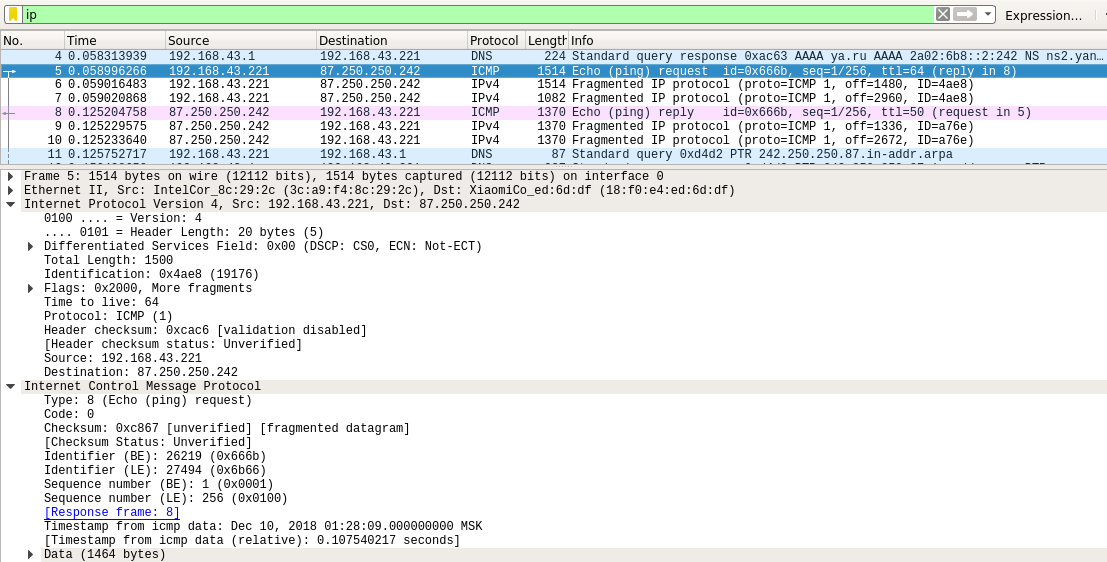
\includegraphics[width=0.95\linewidth]{icmp/ping_frag_request_1.png}
\end{figure}
\vspace{-1.8em}
\begin{figure}[H]
	\centering
	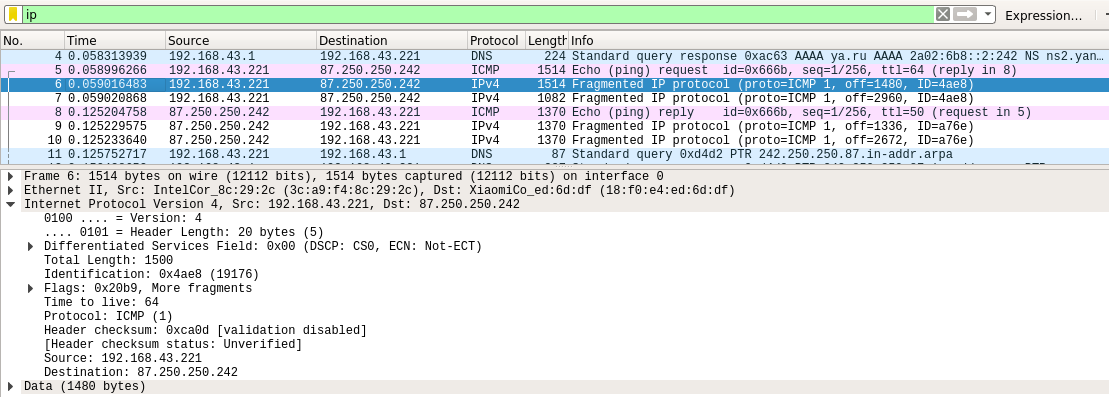
\includegraphics[width=0.95\linewidth]{icmp/ping_frag_request_2.png}
\end{figure}
\vspace{-1.8em}
\begin{figure}[H]
	\centering
	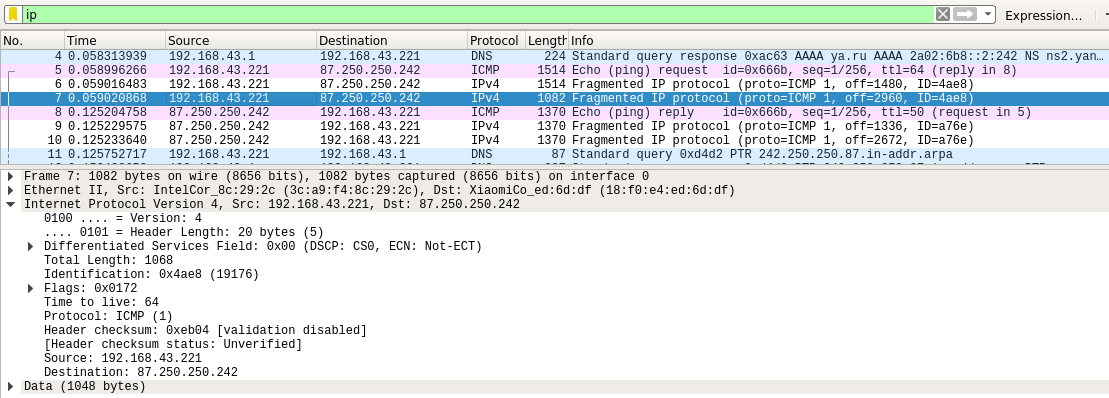
\includegraphics[width=0.95\linewidth]{icmp/ping_frag_request_3.png}
\end{figure}

Видно, что 4 КБ запрос был разбит на 3 пакета размером 1514 Б, 1514 Б и 1002 Б соответственно. ICMP-заголовок присутствует только в первом пакете и поэтому WireShark не определяет остальные пакеты как ICMP-запросы. Кроме того, в фрагментированных пакетах добавляются флаги в IP-заголовок, содержащие информацию о фрагментации (во втором пакете установлен флаг \code{More fragments}, а в последнем пакете нет).

\begin{figure}[H]
	\centering
	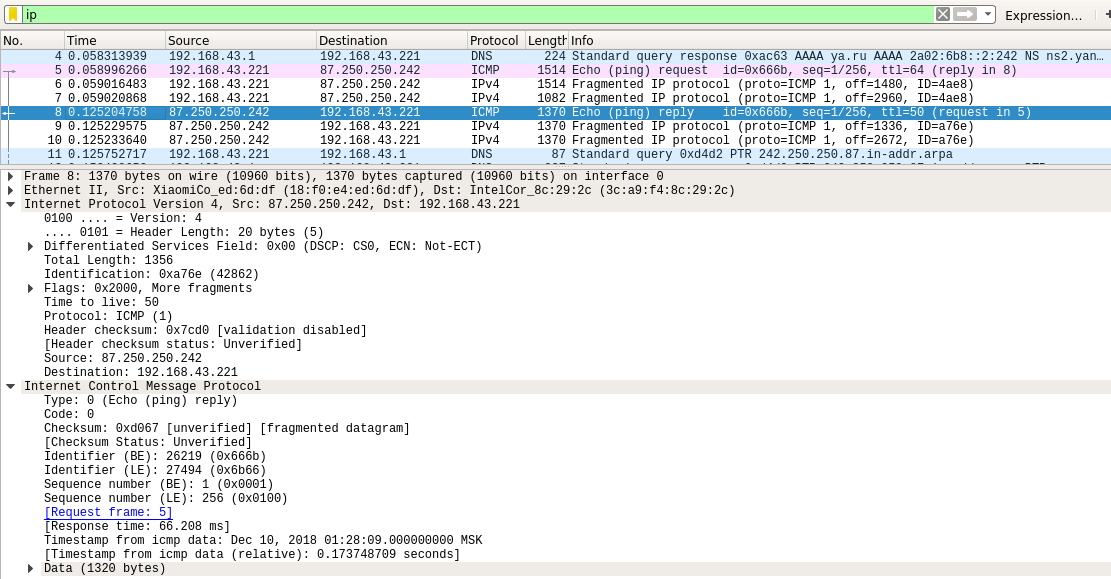
\includegraphics[width=0.95\linewidth]{icmp/ping_frag_response_1.png}
\end{figure}
\vspace{-1.8em}
\begin{figure}[H]
	\centering
	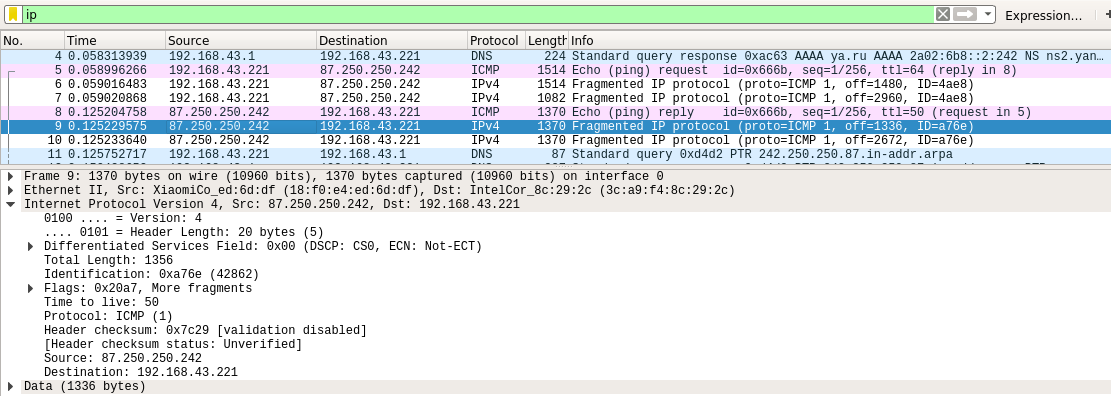
\includegraphics[width=0.95\linewidth]{icmp/ping_frag_response_2.png}
\end{figure}
\vspace{-1.8em}
\begin{figure}[H]
	\centering
	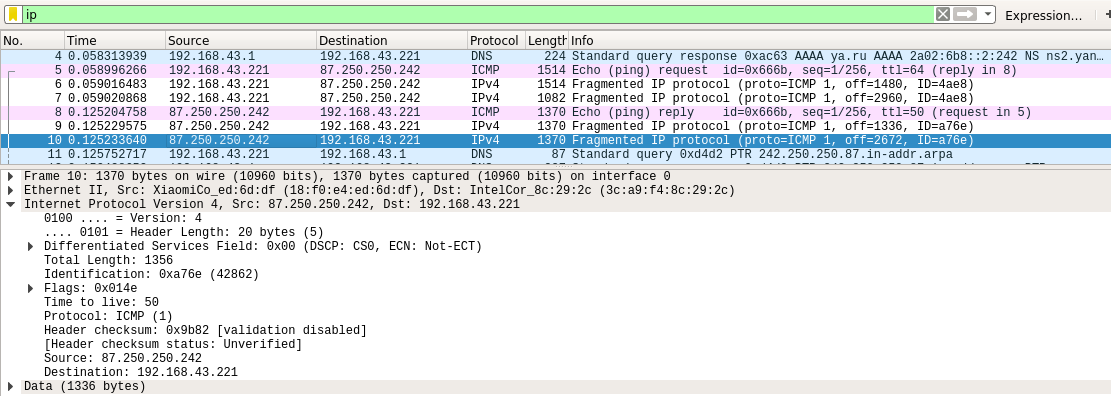
\includegraphics[width=0.95\linewidth]{icmp/ping_frag_response_3.png}
\end{figure}

Был получен фрагментированный ping-ответ. Видно, что было получено 3 пакета, то есть ответ был также фрагментирован. Ping-ответ содержит данные, полностью совпадающие с данными, отправленными в запросе. Аналогично запросу, пакеты содержат флаги с информацией о фрагментации (во втором пакете установлен флаг \code{More fragments}, а в последнем пакете нет).

\end{document}
